\chapter{Исследование решения}
\label{chap:research}

    \section{Описание эксперимента} \\ 
        \paragraph{Предобработка данных}
        \noindent 
        
        \noindent
        \begin{enumerate}
            \item Выделение преамбул из RAW сигналов
            \item Деление преамбул на поля
            \item Параллельная обработка полей преамбул:
            \begin{enumerate}
                \item FFT
                \item Модуль от преобразования Фурье
                \item Выделение значимых частей спектра
                \item Попарное вычитание частей спектра (последний элемент из первого и так далее)
            \end{enumerate}
            \item Конкатенация полученных разностей в один датасет
            \end{enumerate} 
            \begin{figure}[h!]
                \centering
                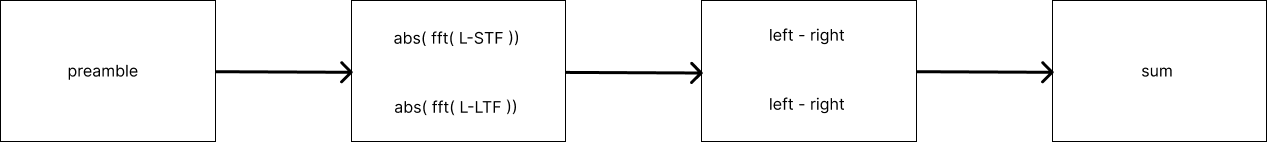
\includegraphics[scale=0.5]{pictures/algh.png}
                \caption{Алгоритм предобработки данных}
                \label{fig:my_label}
            \end{figure} 
             \begin{figure}[h!]
            \centering
            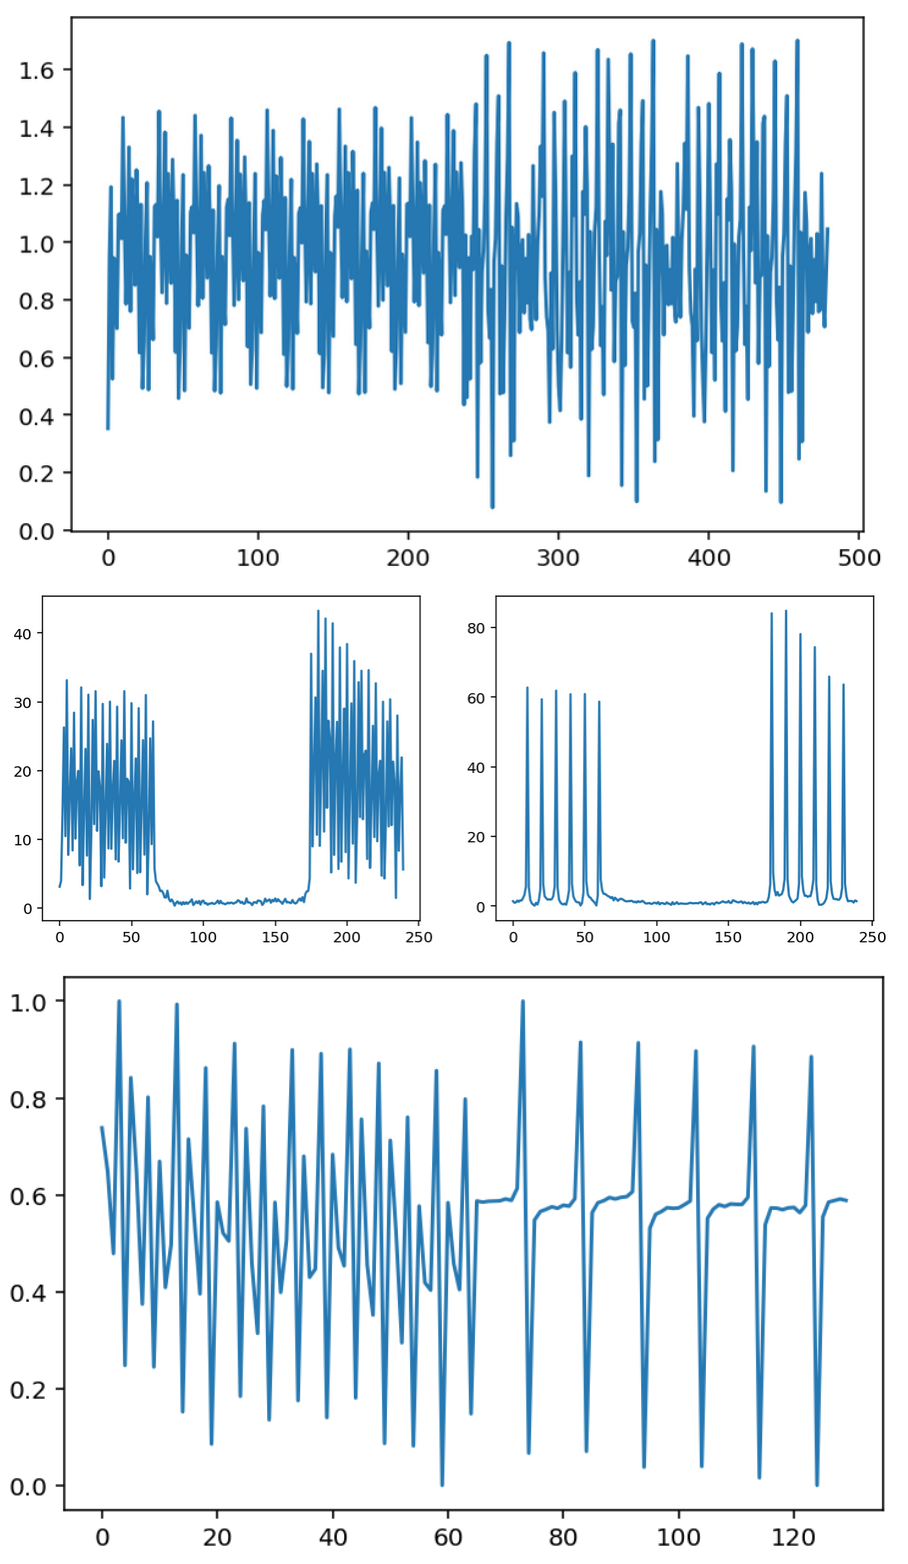
\includegraphics[scale=0.61]{pictures/preproc.png}
            \caption{Результаты обработки, соответствующие шагам 1, 2 и 4
            }
            \label{fig:my_label}
        \end{figure}
            \par
             
        \newpage
        \paragraph{Кодирование/отбор признаков}
        \noindent 
        
        \noindent
        \begin{enumerate}
            \item Отбор признаков с помощью Random Forest
            \begin{enumerate}
                \item Обучение Decision Tree, подбор гиперпараметров
                \item Построение Random Forest на основе обученного дерева решений
                \item Обучение Random Forest
                \item Вызов метода .feature\_importances\_
                \item Сортировка 
                \item Подбор оптимального количества признаков
                \item Оценка результата
            \end{enumerate}
            
            \item Уменьшение размерности признакового пространства с помощью встроенного в MATLAB автоэнкодера
            \item Построение автоэнкодера на основе библиотеки Keras
            \begin{enumerate}
                \item Выбор количества слоев и их размеров
                \item Выбор функций активации
                \item Подбор необходимой комбинации слоев и функций
                \item Оценка результата \\
            \end{enumerate}
            \item TSNE –– проекция выборки на двухмерное пространство для визуализации, а также получения новой информации о данных
            \begin{figure}[h!]
                \centering
                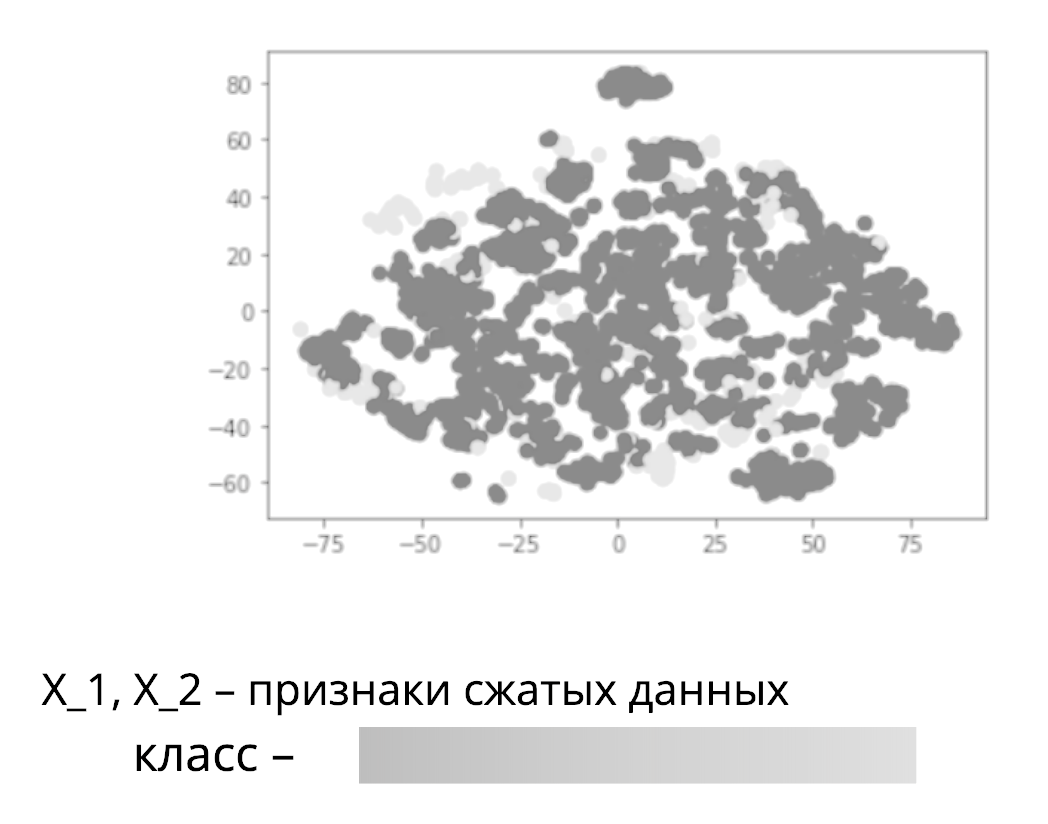
\includegraphics[scale=0.5]{pictures/tsne.png}
                \caption{TSNE
                }
                \label{fig:my_label}
            \end{figure} 
        \end{enumerate} 
        \newpage
        \paragraph{Классификация}
        %сценарий: данные, величины, последовательность действий, гипотезы
        \noindent 
        
        \noindent
        \begin{enumerate}
            \item Decision Tree
            \begin{enumerate}
                \item Кросс-валидация
                \item Обучение
                \item Оценка результатов
            \end{enumerate}
            \item Random Forest
            \begin{enumerate}
                \item Кросс-валидация
                \item Обучение
                \item Оценка результатов
            \end{enumerate}
            \item Multilayer Perceptron
            \begin{enumerate}
                \item Кросс-валидация
                \item Обучение
                \item Оценка результатов
            \end{enumerate}
            \item CatBoostClassifier
            \begin{enumerate}
                \item Кросс-валидация
                \item Обучение
                \item Оценка результатов
            \end{enumerate}
        \end{enumerate}
        
        \paragraph{Адаптация алгоритма}
            \begin{enumerate}
                \item Алгоритм для адаптации – Multilayer Perceptron, как максимально подходящий требованиям к решению
                \item Данные берутся по 300 отсчетов --  batch
                \item Обучение происходит постепенно -- N epochs
                \item После достижения локального взвешенного максимума подается только тестовая выборка
            \end{enumerate}
        
        \newpage
        \paragraph{Технические характеристики} 
\\
         \begin{itemize}
             \item MacBook Pro 13 2015
             \item Процессор 2.7 GHz 2-ядерный Intel Core i5
             \item Память 8 ГБ 1867 MHz DDR3 \\
         \end{itemize}
        %методика измерения: хар-ки пк, инструменты измерения
        \paragraph{Программные средства}
        \begin{itemize}
             \item Язык программирования Python 3.10
             \item Jupyter notebook
             \item Jupyter lab
             \item Atom + Terminal
             \item Graphix
             \item MATLAB 
             \item Библиотеки:
             \begin{itemize}
                 \item Scikit-learn
                 \item Numpy
                 \item Pandas
                 \item MatPlotLib
                 \item SciPy
                 \item TensorFlow
                 \item Keras
                 \item PyTorch
                 \item Seaborn
                 \item CatBoost
                 \item CatBoostClassifier \\
             \end{itemize}
         \end{itemize}
        %используемые программные средства
        
    \newpage
    \section{Результаты}
        \paragraph{Выбор признакового описания}
        \noindent 
        
        
        \begin{table}[h!]
        \centering
        \resizebox{550}{!}{
        \begin{tabular}{l|ccccl|cccl|cccl|lll}
        \cline{2-14}
                   & \multicolumn{5}{c|}{Preambule}                                                                                               & \multicolumn{4}{c|}{L-STF}                                                                      & \multicolumn{4}{c|}{L-LTF}                                                                      &  &  &  \\ \cline{2-14}
                   & \multicolumn{1}{l|}{real}  & \multicolumn{1}{l|}{imag}  & \multicolumn{1}{l|}{abs}   & \multicolumn{1}{l|}{angle} & abs(fft) & \multicolumn{1}{l|}{real}  & \multicolumn{1}{l|}{imag}  & \multicolumn{1}{l|}{abs}   & abs(fft) & \multicolumn{1}{l|}{real}  & \multicolumn{1}{l|}{imag}  & \multicolumn{1}{l|}{abs}   & abs(fft) &  &  &  \\ \cline{1-14}
                    \multicolumn{1}{|l|}{Accuracy} & \multicolumn{1}{c|}{0.732} & \multicolumn{1}{c|}{0.733} & \multicolumn{1}{c|}{0.842} & \multicolumn{1}{c|}{0.702} & 0.828    & \multicolumn{1}{c|}{0.734} & \multicolumn{1}{c|}{0.731} & \multicolumn{1}{c|}{0.838} & 0.785    & \multicolumn{1}{c|}{0.725} & \multicolumn{1}{c|}{0.728} & \multicolumn{1}{c|}{0.836} & 0.822    &  &  &  \\ \cline{1-14}
                    \multicolumn{1}{|l|}{F1-score} & \multicolumn{1}{c|}{0.667} & \multicolumn{1}{c|}{0.663} & \multicolumn{1}{c|}{0.823} & \multicolumn{1}{c|}{0.597} & 0.803    & \multicolumn{1}{c|}{0.668} & \multicolumn{1}{c|}{0.664} & \multicolumn{1}{c|}{0.819} & 0.744    & \multicolumn{1}{c|}{0.646} & \multicolumn{1}{c|}{0.653} & \multicolumn{1}{c|}{0.812} & 0.796    &  &  &  \\ \cline{1-14}
        \end{tabular}}
        \caption{}
        \label{tab:my-table}
        \end{table}
        В Таблице 1 находятся результаты оценки Random Forest различных преобразований данных.
        \begin{table}[h!]
            \begin{tabular}{l|c|c|c|l}
                \cline{2-4}
                                               & L-STF + L-LTF & L-STF & L-LTF &  \\
                                               \cline{1-4}
                \multicolumn{1}{|l|}{Accuracy} & 0.85          & 0.83  & 0.84  &  \\ \cline{1-4}
                \multicolumn{1}{|l|}{F1-score} & 0.83          & 0.81  & 0.83  &  \\ \cline{1-4}
            \end{tabular}
            \caption{Оценка для L-STF, L-LTF и их суммы}
            \label{tab:my-table}
        \end{table}
        
        Таблица 2 – сравнительная таблица F1-score и Accuracy на классификаторе Random Forest для полей L-STF, L-LTF и их суммы, прошедших выбранную схему преобразования.\\ Очевидно, что L-LTF вносит больший вклад в решение задачи классификации, чем L-STF, но их сумма показывает большую точность.
        
        \begin{figure}[h!]
            \centering
            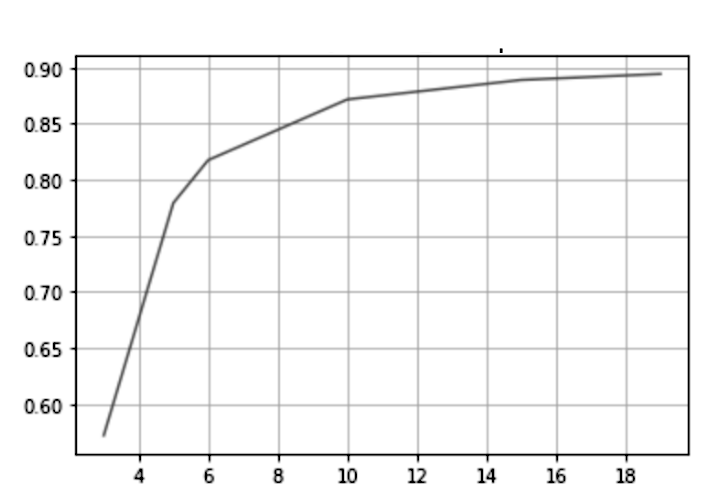
\includegraphics[scale=1]{pictures/acc_nf.png}
            \caption{Точность от количества признаков
            }
            \label{fig:my_label}
        \end{figure} 
        
        На рис. 15 изображена зависимость Accuracy от количества признаков в выборке. Эти признаки отобраны по значимости, рассчитанной Random Forest. \\Можно заметить, что начиная с 10 признаков Accuracy меняется незначительно, то есть это значение оптимально.
        
        \newpage
        \begin{figure}[h!]
            \centering
            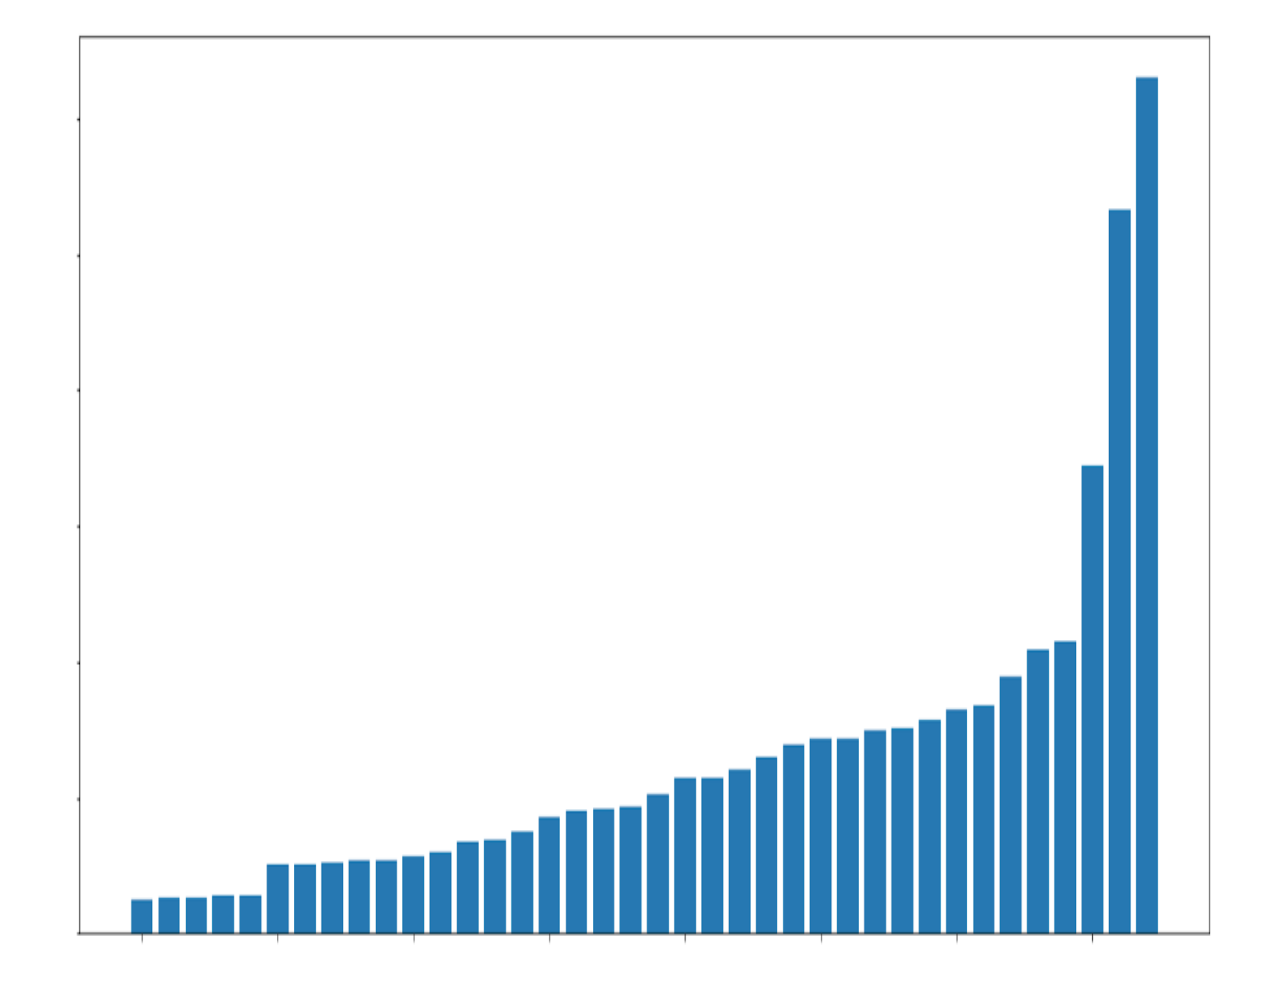
\includegraphics[scale=0.5]{pictures/RF-ff.png}
            \caption{Средний вклад в изменение энтропии от признака
            }
            \label{fig:my_label}
        \end{figure} 
        
        На рис. 16 изображено распределение признаков выборки по их значимости, рассчитанной Random Forest.\\ Признаки расположены в порядке возрастания значимости -- среднего вклада в изменение энтропии при построении дерева.\\
        
        \paragraph{Точность классификации \\} \\
        \noindent
        \begin{table}[h!]
        \begin{tabular}{l|l|l|l}
        \cline{2-3}
                                                          & Accuracy & F1-score &  \\ \cline{1-3}
        \multicolumn{1}{|l|}{Decision tree}               & 0.81     & 0.73     &  \\ \cline{1-3}
        \multicolumn{1}{|l|}{Random forest}               & 0.86     & 0.78     &  \\ \cline{1-3}
        \multicolumn{1}{|l|}{CatBoost Classifier}         & 0.95     & 0.88     &  \\ \cline{1-3}
        \multicolumn{1}{|l|}{Autoencoder + Random forest} & 0.85     & 0.83     &  \\ \cline{1-3}
        \multicolumn{1}{|l|}{Autoencoder + MLP}           & 0.92     & 0.91     &  \\ \cline{1-3}
        \multicolumn{1}{|l|}{Autoencoder + CatBoost}      & 0.91     & 0.90     &  \\ \cline{1-3}
        \end{tabular}
        \caption{Таблица классификаторов}
        \label{tab:my-table}
        \end{table}
        В таблице 3 указаны оценки классификаторов в различных конфигурациях. \\Можно заметить, что самые примитивные классификаторы – DT и RF дают неплохой результат, но не полностью отвечают сформулированным требованиям. Лучшими комбинациями являются Autoencoder+MLP и Autoencoder+CatBoost.
        \newpage
        \paragraph{Сравнительный анализ}
        \noindent\\
        Рассмотрим подробнее классификаторы CatBoostClassifier и MLPClassifier.
        
        \begin{figure}[h!]
                \centering
                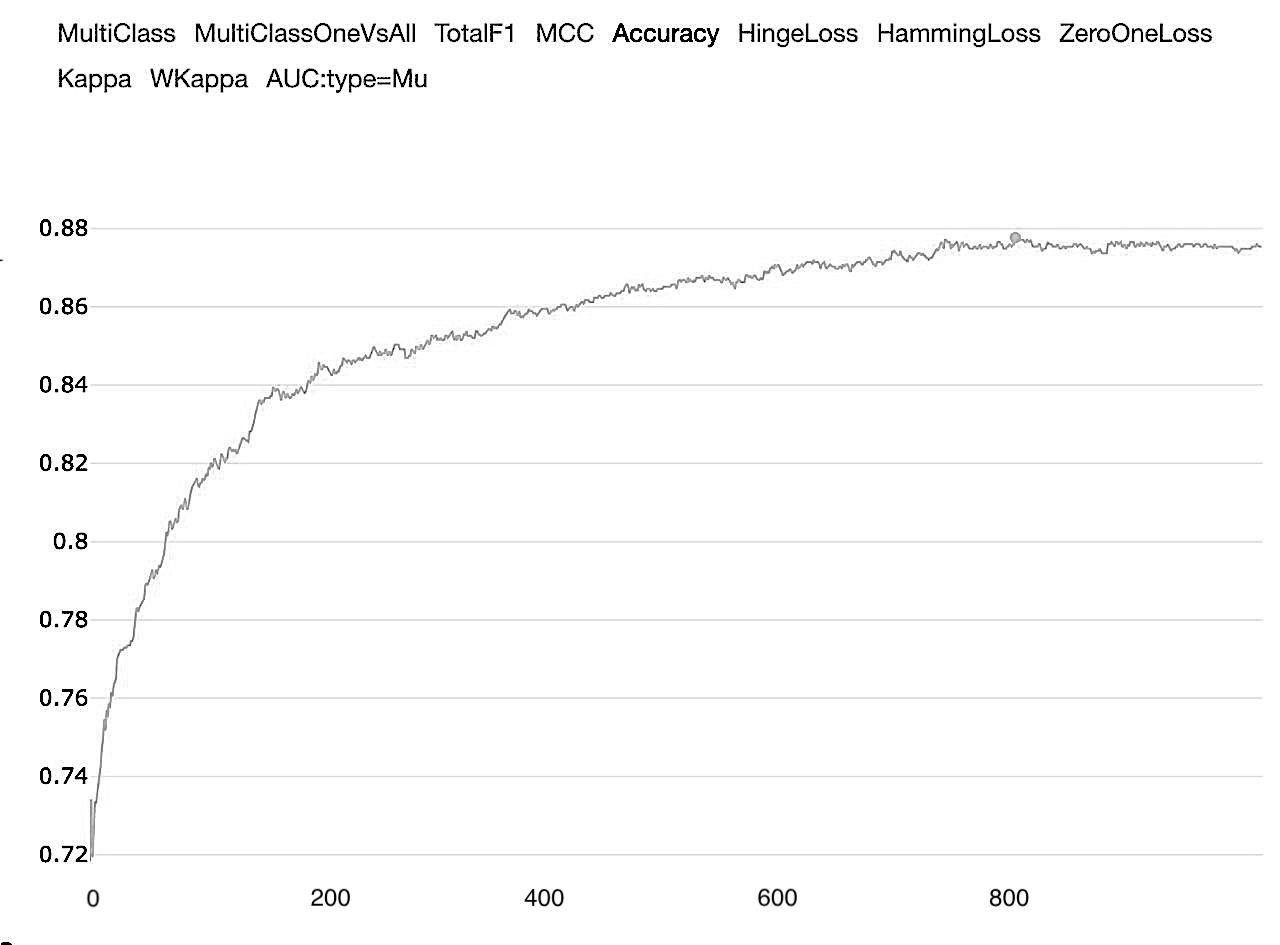
\includegraphics[scale=0.2]{pictures/2022-06-21 02.22.10.jpg}
                \caption{CatBoostClassifier
                }
                \label{fig:my_label}
            \end{figure} 
        \begin{figure}[h!]
                \centering
                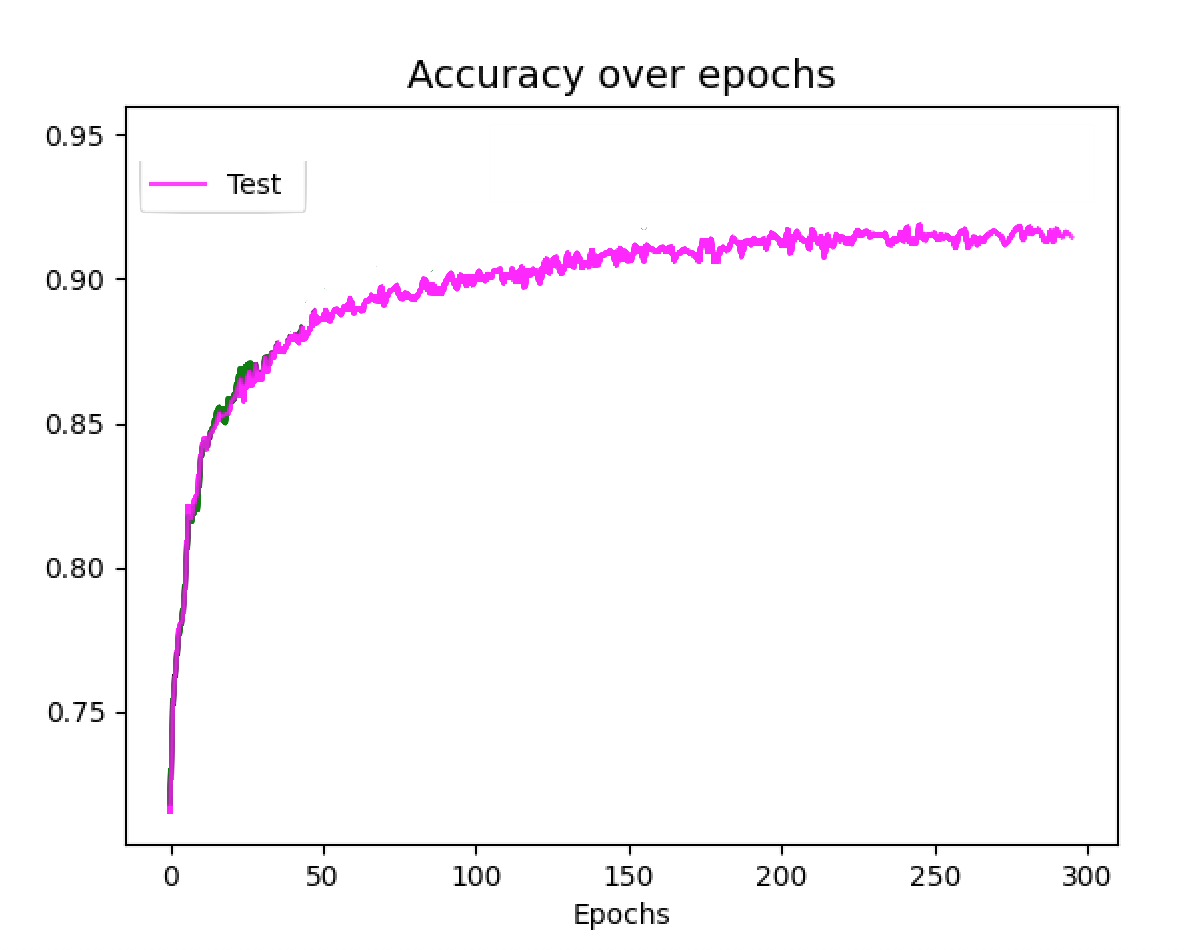
\includegraphics[scale=0.5]{pictures/realtime.png}
                \caption{Multylayer Perceptrone
                }
                \label{fig:my_label}
            \end{figure} 
            Оба алгоритма сходятся, CatBoost – к 0.88, а MLP – к 0.91, при этом оба работают в режиме реального времени.
        \noindent
        \paragraph{Выводы}
        
        \begin{itemize}
            \item Лучшее признаковое пространство получено преобразованиями+автоэнкодером
            \item Самую высокую точность показал многослойный персептрон
            \item Задача классификации решается композицией вышеназванных алгоритмов в онлайн-режиме со стабильной точностью
        \end{itemize}
        \noindent
        